\documentclass[useAMS,usenatbib,bibyear]{aa}
\def\pdf{1} % 0 for eps, 1 for pdf
\usepackage{txfonts}
\usepackage{epsfig,amsmath,mathrsfs}
\usepackage{natbib}
\bibpunct{(}{)}{;}{a}{}{,} % to follow the A&A style

\ifnum\pdf=0 \usepackage[dvips,usenames,dvipsnames]{color} \fi
\ifnum\pdf=1 \usepackage[usenames,dvipsnames]{color} \fi

\usepackage{graphicx}
%\usepackage{graphics}
\usepackage[]{hyperref} % Had to remove option 'pdftex' from the []'s
\usepackage{fontawesome}
\usepackage{bm}
\usepackage{verbatim}
\usepackage{amssymb}
\usepackage{xcolor}
\usepackage{tikz}
\usepackage[tikz]{bclogo}
\usepackage[framemethod=tikz]{mdframed}
\newcounter{infobox}[section]
\renewcommand{\theinfobox}{\thesection.\arabic{infobox}}
\newenvironment{infobox}[1][]{%
    \refstepcounter{infobox}
    \begin{mdframed}[%
        frametitle={Box \theinfobox\ #1},
        skipabove=\baselineskip plus 2pt minus 1pt,
        skipbelow=\baselineskip plus 2pt minus 1pt,
        frametitleaboveskip= 7pt,
        frametitlebelowskip= 7pt,
        linewidth=0pt,
        linecolor=black,
        frametitlerule=false,
        frametitlebackgroundcolor=blue!10,
        backgroundcolor=blue!10,
        roundcorner=7pt,
    ]%
}{%
    \end{mdframed}
}

\newcommand{\red}[1]{\textcolor{red}{\textbf{#1}}}
\definecolor{gray}{RGB}{180,180,180}
\newcommand{\gray}[1]{\textcolor{gray}{#1}}
\renewcommand{\sec}[1]{Sec.~\ref{sec:#1}}
\def\ergs{\mbox{\,erg~s$^{-1}$}}
\definecolor{DarkRed}{RGB}{195,0,0} % "RGB" -> [0,255]; "rgb" -> [0,1]
\hypersetup{colorlinks,%
            citecolor=blue,%
            filecolor=black,%
            linkcolor=DarkRed,%
            urlcolor=blue}%,%
          % pdftex}

\usepackage{pgfornament}

\begin{document} 

\title{Multiplicity of timescales: Insight into galaxy formation}
\author{Peter Laursen\inst{1,2}}
\institute{Cosmic Dawn Center (DAWN).
  \email{pela@nbi.ku.dk}.
  \and
  Niels Bohr Institute, University of Copenhagen, Jagtvej 128, 2200 Copenhagen N, Denmark.
  }
\date{\today}
\abstract{Timescales in astronomy comprise the largest range of any scientific discipline.
In the construction of physical models, this circumstance may both be a blessing and a curse.
For example, galaxy evolution occurs on typical timescales of hundreds of millions of years, but is affected by atomic processes on sub-second timescales, posing a serious challenge in analytical and, in particular, in numerical models.
On the other hand, the vast dynamic range implies that we can often make meaningful predictions by simply comparing characteristic timescales of the physical processes involved.
This brief review, aimed primarily at non-astronomer scientists, attempts to highlight a few occasions in the context of galaxy formation and evolution in which comparing timescales can shed light on astrophysical phenomena, as well as some of the challenges that may be encountered.}
\keywords{galaxies: kinematics and dynamics --- galaxies: formation --- cosmology: theory.}

\maketitle

\section{Introduction}
\label{sec:intro}

No scientific field deals with a longer span of timescales than astrophysics.
From explosion mechanisms in dying stars and oscillations of neutron stars, to cosmic structure formation and the age of the Universe itself, more than twenty orders of magnitude prevail.
Counting Big Bang physics as ``astrophysics'' doubles or even triples this amount\footnote{ The age of the Universe is $\sim10^{61}$ Planck times!}.
However, while this enormous dynamic range can be challenging to model under one umbrella, it may also be an advantage: Because the evolution of a system in general happens at a rate determined by the longer timescale, modified by shorter timescales, many characteristic features of various astrophysical phenomena can be understood simply by comparing relevant physical timescales.

Whereas the short end of this range of timescales is in many cases observable, an inherent problem in astronomy is that many processes occur on timescales much longer than a human life, or even a human civilization that would be able to pass knowledge down through generations.
How, then, may we say anything about how stars form, how galaxies evolve, or which phases the Universe has gone through?

Several approaches exist to answering this question: Observationally, while we cannot wait to witness the evolution of any given galaxy --- which to us puny humans appears frozen in time --- we are lucky to live in a universe where the speed of light is finite, but fast.
As we peer deeper into the cosmos, we probe earlier and earlier epochs.
Observing large samples of galaxies throughout cosmic history then allows us to study their properties in a statistical sense --- numerous defining properties such as their star formation rates, the build-up of heavy elements and dust, and changes in their morphology.

On the theoretical side, as in all other fields of science we make use of \emph{models}.
Models that predict the evolution of these various physical properties, while being (largely) consistent with already known physical properties.
Models can be analytical, numerical, or a mixture thereof; the so-called semi-analytical models.
In this chiefly theoretical review we will have a look at how timescales can be used to make meaningful predictions about the most beautiful structures in the Universe; the galaxies.

Ever since the revelation that the Milky Way does not comprise the whole Universe, but that we are surrounded by countless similar ``island universes'' \citep{Shapley1921,Hubble1926}, we have strived to comprehend the origin of these magnificent entities.
Which physical processes may lead to their formation and govern their evolution, while at the same time resulting in the astounding observed heterogeneity in their properties?

Progress in this captivating field is not only an exquisite interplay between
the increasing power of telescopes and detectors,
improved observational techniques,
and an increasingly better theoretical understanding of cosmology and the Universe in general;
advances are also stimulated by breakthroughs in such diverse fields as particle physics, chemistry, and computer science.
No man is an island \citep{Jovi1990}, and indeed the same is true for fields of science --- interdisciplinarity is essential to progress!

\section{Galaxy formation and evolution}
\label{sec:galaxies}

A brief outline of the physical processes leading to a galaxy can be summarized as follows:

In the early, expanding Universe, sufficiently large overdensities are able to withstand and detach themselves from this expansion, turn over, and collapse.
With more than five times as much dark matter as baryonic matter, the dynamics are initially dominated by the former.
Eventually the cloud will \emph{virialize} --- astronomers' term for reaching a dynamical equilibrium --- and come to a halt.
Gas, which unlike the collisionless dark matter is able to cool and fragment further, condenses in the center of more extended dark matter halos.

In the very center, supermassive black holes form which accrete mass, ejecting excess energy as so-called \emph{active galactic nuclei} (AGN).
Meanwhile, dying stars inject not only energy but also heavy elements (in astronomy, everything heavier than helium is collectively called ``metals'').
With time, the interstellar medium (ISM) is therefore enriched with metals, part of which condenses to dust.

Thermal and kinetic feedback from stars and AGN drive strong winds which may exceed the galaxy's escape velocity, enriching also the intergalactic medium (IGM) with metals.
Star formation typically declines after an initial starburst, but may be sustained by continuous accretion of new material from the IGM, while new starbursts may be initiated by collisions with other galaxies, a process known as \emph{merging}.
Galactic winds, merging, and gas depletion is also responsible for some galaxies ceasing to form new stars.

Which processes dominate will determine the nature of the galaxy, in particular its color and its morphology: will it end up as a disky spiral galaxy, a featureless elliptical galaxy, or something else?

% \noindent\fcolorbox{darkgray}{lightgray}{%
\begin{figure}[!t]
\minipage[t!]{\dimexpr0.98\linewidth-2\fboxsep-2\fboxrule\relax}
\begin{bclogo}[
    couleur=gray!20,
    epBord=1,
    arrondi=0.1,
    logo=\bcinfo,
    marge=8,
    ombre=false, %true,blur,
    couleurBord=gray!60,
    barre=line]
    { \ \textsf{Cosmological redshift}}
    \small{\textsf{Arguably, the most essential concept in astronomy is the \emph{redshift} of light, denoted by the letter $z$.
    Well-known to other physicists as \emph{Doppler shift}, the result of a relative motion between emitter and observer, in extragalactic astronomy there is second effect, dominating on all but the most local scales, caused by the cosmological expansion of the Universe.\vspace{1mm}\\
    As light travels through expanding space, its wavelength increases by a factor $1+z$, equal to the ratio of the size of the Universe at the time of observation and emission, respectively.
    Because the Universe has always been expanding, the observed redshift becomes a measure of both the age of the Universe at emission, the current distance, the ``lookback time'', the observed volume, and several other useful aspects.
    We therefore simply use the term redshift to talk about all these quantities, collectively.
    For instance, we refer to galaxy seen 1 billion years after the Big Bang as ``\emph{a redshift 2 galaxy}'', we observe ``\emph{the high-$z$ Universe}'' (with disparate definitions among different researchers), or we speak of ``\emph{the evolution of galaxies with redshift}''.\vspace{1mm}\\
        Because the Universe was smaller in the past, the relative expansion of the Universe decreases.
        Hence, the time span between, say, $z=0$ (today) and $z=1$ is much longer than between $z=10$ and $z=11$, namely 8 billion years (Gyr) and 60 million years (Myr), respectively.
        Partly for the same reason, however, the timescales of evolution --- not only of galaxies but for all physicall processes --- were shorter at earlier times.\vspace{1mm}\\
        The relationship between redshift and other quantities is shown in Fig.~\ref{fig:redshift}.
    }}
\label{info:redshift}
\end{bclogo}
     \endminipage
     %}\hfill
\end{figure}

\begin{figure}[!t]
    \begin{center}
        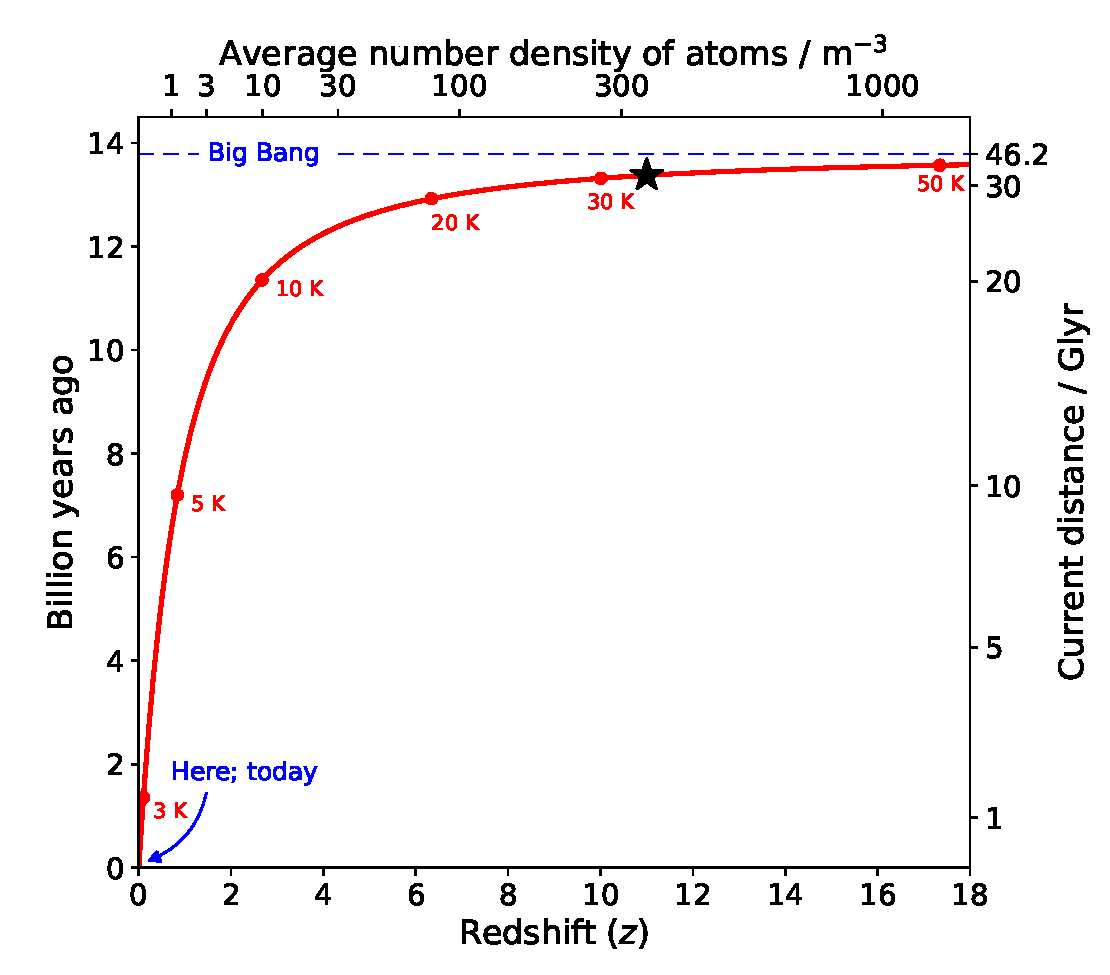
\includegraphics[width=0.98\linewidth]{redshift.pdf}
        \caption{Relationship between observed redshift of light emitted from a distant object, and various properties of the Universe.
        Because the relative expansion was larger in the past when the Universe was smaller, redshift increased more at that time asymptotically approaching infinity for light emitted at the time of the Big Bang, 13.8 Gyr ago.
        The red dot marks the current record for the most distant known galaxy, GN-z11, with $z=11.09$ \citep{Oesch2016}.}
        \label{fig:redshift}
    \end{center}
\end{figure}

\subsection{The luminosity function}
\label{sec:LF}

One of most popular ways of describing statistically a population of galaxies and its evolution through cosmic time is the \emph{luminosity function} (LF) --- the probability distribution function of the luminosities of galaxies in a given wavelength band, e.g. rest-frame ultraviolet light.
Carefully taking into consideration observational pitfalls such as differential dust extinction and various selection biases (e.g.~faint galaxies are progressively more difficult to see at high redshift than bright galaxies), the physical properties and the evolution of a given galaxy type can then be studied through time.

All structure in the Universe is, ultimately, born out ouf primordial (quantum) fluctuations in the density field.
Observations of the cosmic microwave background (CMB) show that apparently these fluctuations can be described by an almost scale-free power spectrum \citep{PlanckCollaboration2018a}.
In other words, the Universe does not have a preferred scale, and neither does gravity (there are no characteristic masses in the Einstein equations).
We might therefore expect structure to form in a self-similar way: If the ratio between the number of structures with masses $M$ and $10M$ is $f$, then the ratio between the number of structures with masses $\frac{1}{10}M$ and $M$ is also $f$.
%Stars are born with a distribution of masses, and hence with a distribution of luminosities.
%Assuming a given distribution at their birth, the so-called \emph{initial mass function} (IMF), allows us to convert the luminosity at a given wavelength (e.g.~``the UV region'' or ``the H$alpha$ line'') to a stellar mass.
And if all halos contain the same baryonic fraction and are equally effective at converting gas to stars, we might expect the LF to reflect the distribution of masses in the Universe.

The Universe, it turns out, is more complex than this, as will be elucidated further down.
Observationally, we do however see a LF that is remarkably universal --- that is, it can be rather accurately parametrized by same functional form for all galaxy types, and all redshifts:
As seen in Fig.~\ref{fig:LF}, at low luminosities the LF is characterized by a power law, while above a certain characteristic luminosity there is an exponential cut-off.
Observed luminosities are therefore often fitted with a so-called Schechter function \citep{Schechter1976} with three parameters that are a function of redshift: The faint-end slope $\alpha$, the normalization $\phi^*$, and the ``knee'' luminosity, $L^*$ (pronounced ``L-star''):
\begin{equation}
    \label{eq:LF}
    N(L)dL=\phi^* \left({\frac{L}{L^*}}\right)^{\alpha} e^{-L/L^*}{\frac{dL}{L^*}}.
\end{equation}
\begin{figure}[!t]
    \centering
    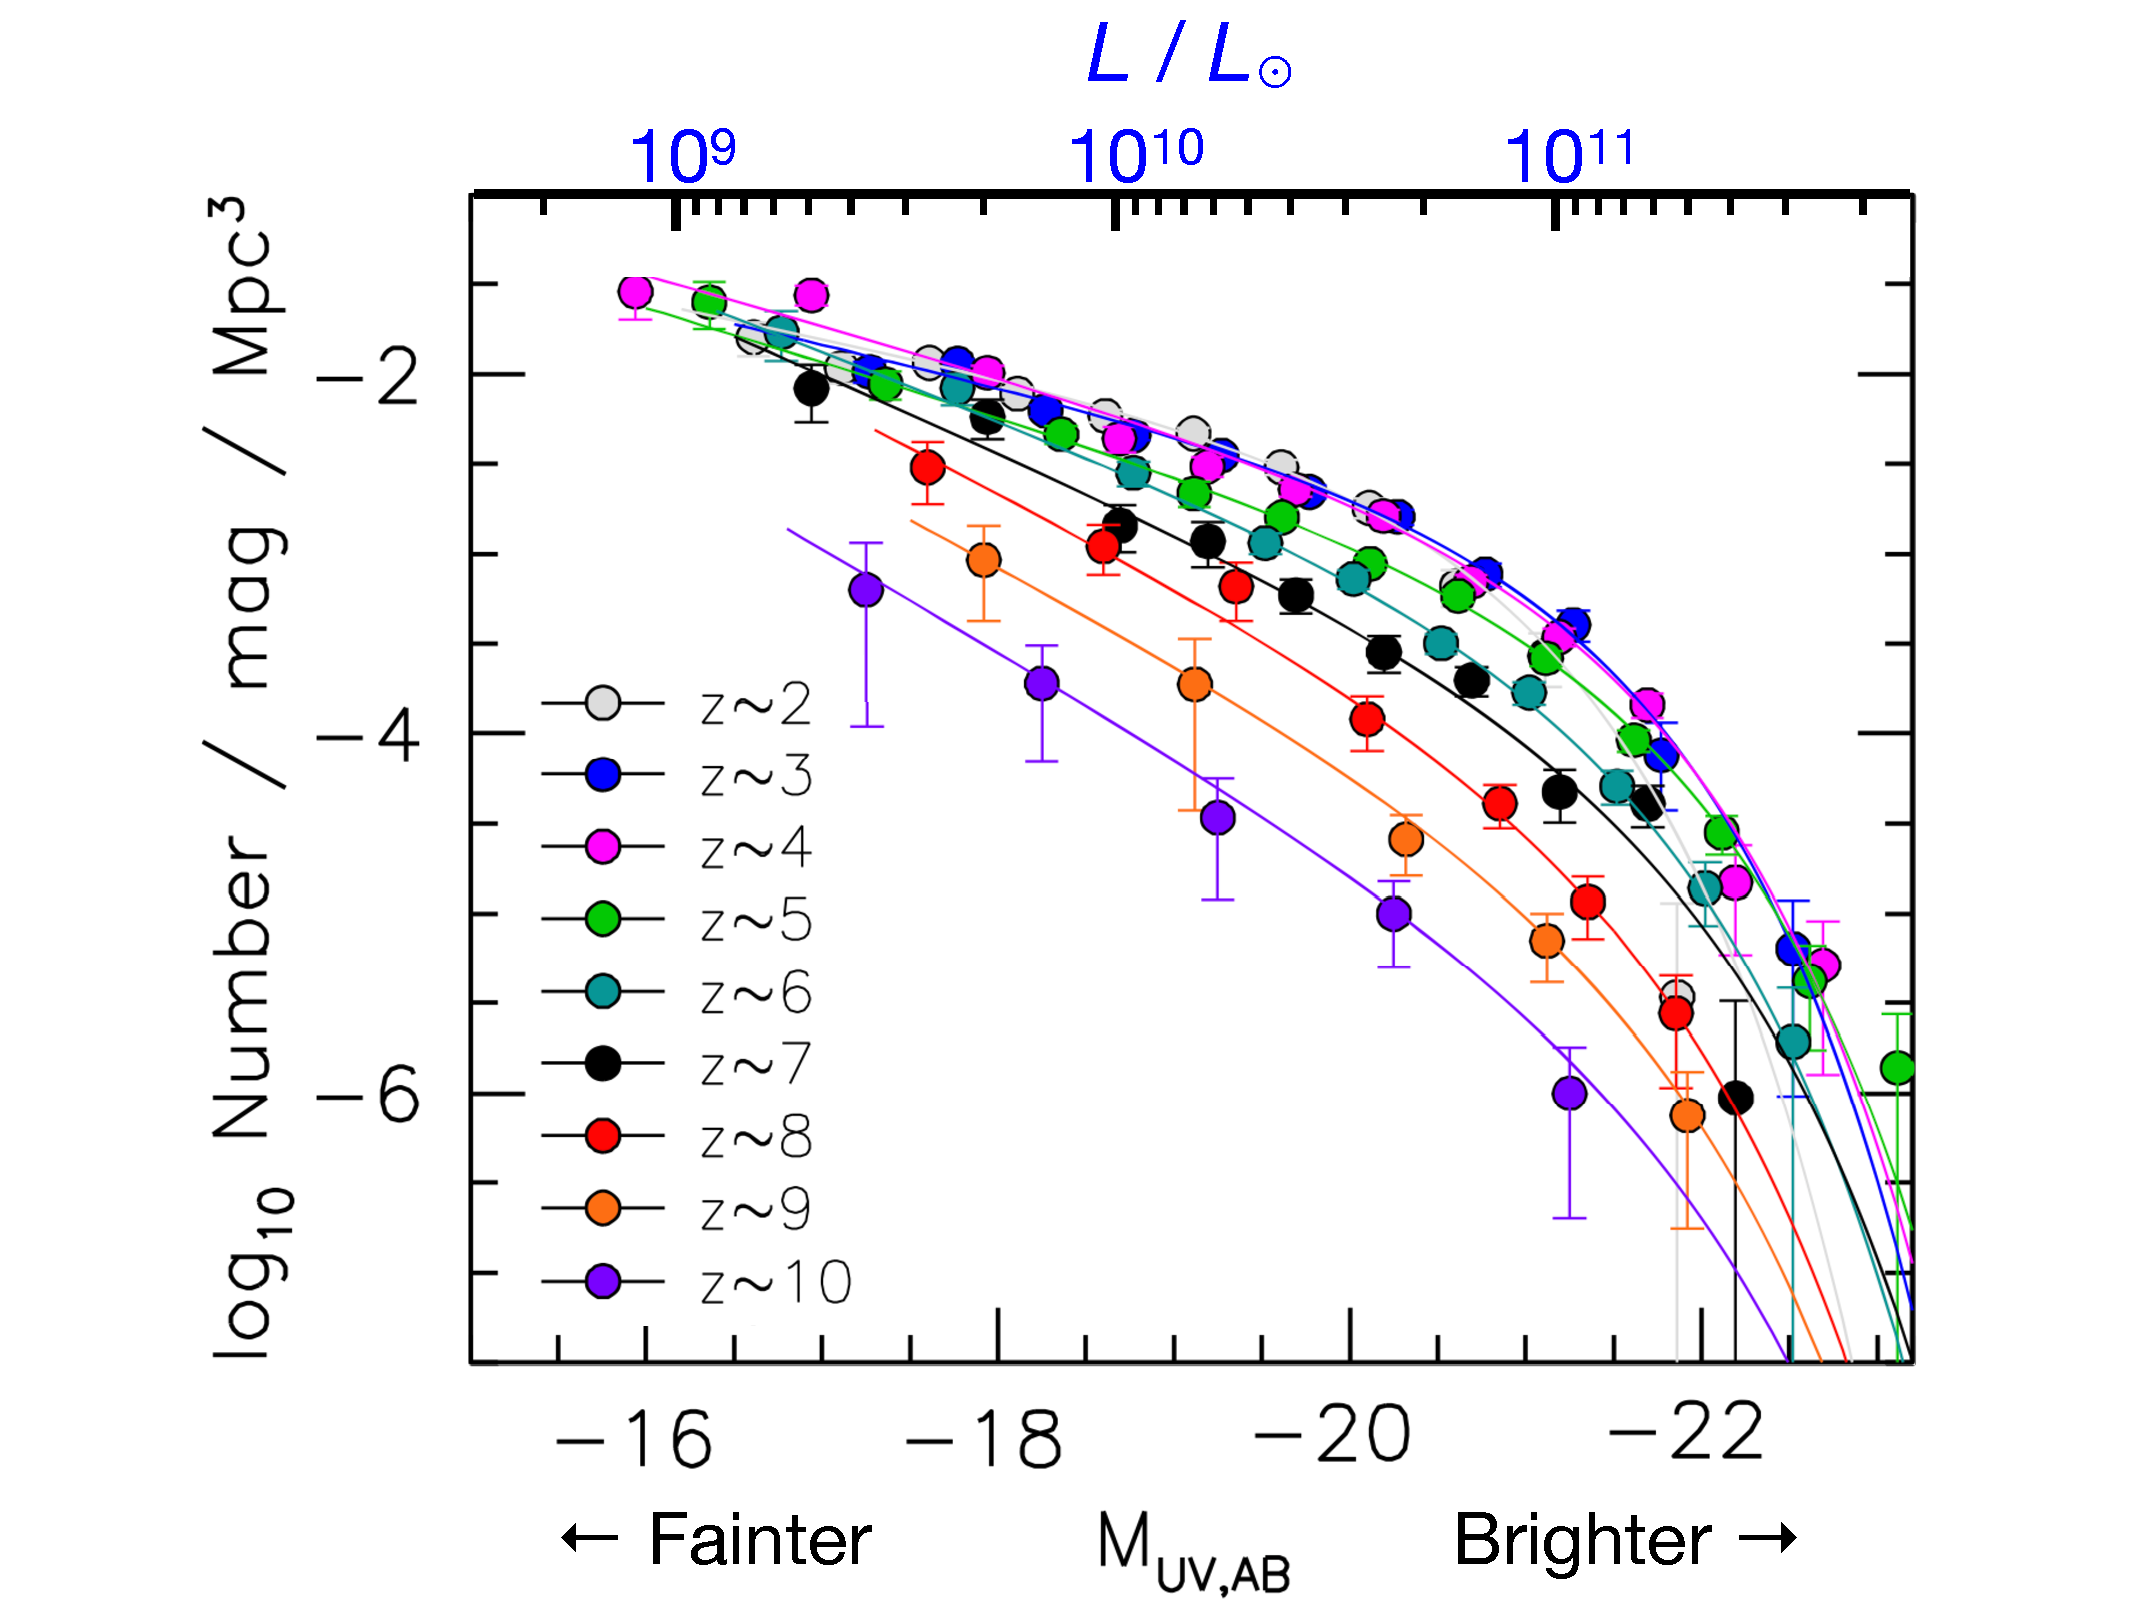
\includegraphics [width=0.48\textwidth] {bouwens2021.pdf}
    \caption{The evolving (ultraviolet) luminosity function of galaxies from the Universe was $\sim500\,\mathrm{Myr}$ ($z\sim10$) till it was $3.3\,\mathrm{Gyr}$ old ($z\sim2$).
    Along the $y$ axis is differential number density, while the luminosity along the $x$ axis is given in Solar luminosities.
    The data for $z\sim10$ is from \citet{Oesch2018}, while the rest is taken from \citep{Bouwens2021}.
    The lines show the best-fit Schechter functions (Eq.~(\ref{eq:LF})).}
    \label{fig:LF}
\end{figure}
The cut-off implies that there is in fact such a thing as a ``typical galaxy'', roughly comparable to our own Milky Way.
The fact that the number density of galaxies larger than the Milky Way declines exponentially fast means that, if one integrates the total stellar mass of all galaxies, Milky Way-sized galaxies dominate the total stellar budget in the Universe.
It is thus not entirely coincidental that we live in an $L^*$ galaxy, although other factors than just the sheer number of stars are important (not all galaxies are equally habitable).

The evolution of the LF with time has proved an invaluable tool for teaching us how galaxies have evolved since their formation.
Unlike earlier attempts to characterize galaxy populations, the Schechter function is not purely phenomenological, but has its roots in the underlying distribution of matter.
In the following I will attempt to shed light on how from a timescale perspective we can understand, to a certain extent, the physics of the LF.

\subsection{The halo mass function}
\label{sec:HMF}

One of the big discoveries of the 1970s was that, in contrast to the prevailing picture at the time \citep{Eggen1962}, galaxies do not form from huge, ``monolithically collapsing'' clouds that later fragment to stars.
Rather, it seems to be the other way round, with small structures forming first, later building up to larger structures in a hierarchical manner.
This was first realized by \citet{Press1974}, and later refined by e.g. \citet{Sheth2002} and \citet{Tinker2008}, who calculated the collapse of gravitating clouds from an initial smoothed density field.
The resulting \emph{halo mass function} (HMF) is analogous to the LF,
but for DM halo masses rather than galaxy luminosities.
Since baryons and dark matter was originally mixed in the ratio $\sim$1:5, one might expect that the LF would mimic the HMF, albeit shifted to lower masses.
But this is not at all what we see! Although they are both characterized by a power law and an exponential cut-off, the HMF cut-off is at much high masses than the halos hosting $L^*$ galaxies.

The exponential departure of the HMF from a universal power law derives from the Gaussian (or at least near-Gaussian) distribution of clumps in the inital density field.
Structure forms on all scales, but because no information can be gained from outside the cosmic event horizon --- i.e.
the ``boundary'' marking the sphere within which light has had the time to travel since the Big Bang, the so-called ``observable Universe'' --- small structures form before larger ones.
The relevant timescale that sets the maximum size of structures in the Universe at a given time is the \emph{Hubble time}, defined at a time $t$ as $t_\mathrm{H}(t) = 1/H(t)$, where $H(t)$ is the Hubble parameter that measures the expansion rate of the Universe\footnote{The expansion rate measures the recession velocity at a given distance, typically in km/s per Mpc, or ``mega-parsec'', where 1 pc $\simeq$ 3.3 lightyears.
The current value of $H(t)$ is called the Hubble constant, $H_0$, and is roughly equal to $H_0\simeq70\,\mathrm{km}\,\mathrm{s}^{-1}\,\mathrm{Mpc}^{-1}$.}.
If the Universe had always expanded at its current rate, $t_\mathrm{H}$ would be equal to the age of the Universe.
In most cases we can ignore physical processes that happen on timescales longer than $t_{H}$.
For instance, this timescale sets the primordial abundances of elements created through nucleosynthesis in the first 20 minutes after the Big Bang.

\subsection{Gas cooling in dark matter halos}
\label{sec:cooling}

How may we understand the shape of the LF? The first clues to this problem were provided by \citet{Rees1977} who simply compared two timescales: 

A cloud of gas and DM that meets the Jeans criterion and is able to withstand the expansion of the Universe collapses first in a free fall.
In the simple case of a spherically symmetric collapse, all particles of a pressureless gas meet in the center in the free-fall time $t_\mathrm{ff}$ given by
\begin{equation}
    \label{eq:tff}
    t_\mathrm{ff} = \left( \frac{3\pi}{32 G \rho_\mathrm{m}} \right)^{1/2}
                  = \left( \frac{3\pi f_\mathrm{b}}{32 G n \mu m_\mathrm{H}} \right)^{1/2},
\end{equation}
where $G$ is the gravitational constant, and $\rho_\mathrm{m}$ is the mass density. In the early Universe, before dark energy played any role (see info box~\ref{info:expansion}), the density simply evolved as $\rho_\mathrm{m}(z) = \rho_\mathrm{m,0} (1+z)^3$ where $\rho_\mathrm{m,0} = \rho_\mathrm{DM,0} + \rho_\mathrm{b,0}$ is the present-day density.
In the second step we have expressed this density in terms of the gas through the universal baryonic fraction $f_\mathrm{b} = \rho_\mathrm{b}/\rho_\mathrm{m} = 0.16$ \citep{PlanckCollaboration2018a}, the particle density $n$, and the mean molecular mass\footnote{For a primordial gas of hydrogen and helium in the mass ratio $\frac{3}{4}$:$\frac{1}{4}$, the mean molecular mass is 1.23 or 0.59 if the gas is neutral or fully ionized, respectively.} $\mu$ in terms of the hydrogen mass $m_\mathrm{H}$.

% \noindent\fcolorbox{darkgray}{lightgray}{%
\begin{figure}[!t]
\minipage[t!]{\dimexpr0.98\linewidth-2\fboxsep-2\fboxrule\relax}
\begin{bclogo}[
    couleur=gray!20,
    epBord=1,
    arrondi=0.1,
    logo=\bcinfo,
    marge=8,
    ombre=false, %true,blur,
    couleurBord=gray!60,
    barre=line]
    { \ \textsf{Expansion of the Universe}}
    \small{\textsf{
        The Universe consists of several different components which affect its dynamics differently:
        Dark energy (DE) has a constant energy density; more DE is therefore created along with the expansion of the Universe.
        Matter (m) consists of dark matter (DM) and baryons (b) which both act ``normally''; its density decreases proportionally to the volume because the total amount is conserved (except when converted to radiation). Because redshift is inversely proportional to the ``size'' of the Universe, or \emph{scale factor} $a$ --- i.e. the redshift of an object observed when the size of the Universe was $a$ compared to today is given by $1+z=1/a$ --- the density of matter evolves with redshift as
        $\rho_\mathrm{m}(z) = \rho_\mathrm{m,0} (1+z)^3$.
        Radiation (r) may of course be created and destroyed, but the number of photons is dominated by CMB photons which are largely conserved. However, in addition its energy density is diluted due to its redshift, and the energy density therefore goes as
        $\rho_\mathrm{r}(z) = \rho_\mathrm{r,0} (1+z)^4$.\vspace{1mm}\\
        Because of the differing exponents, the different components dominate on different timescales:
        In the very early Universe, dynamics were dominated by radiation until an age of roughly $t = 50\,000\,\mathrm{yr}$, after which we entered the matter-dominated era.
        The future will bring an exponential expansion because DE took over at around $t\sim10\,\mathrm{Gyr}$, but it is a rather remarkable fact that we live in an era where both matter and DE governs the expansion.
    }}
\label{info:expansion}
\end{bclogo}
     \endminipage
     %}\hfill
\end{figure}


But the gas is \emph{not} pressureless, and an initially adiabatic collapse therefore increases the gas temperature until thermal pressure prevents the cloud from contracting further and the gas is shock-heated to the \emph{virial temperature}:
\begin{eqnarray}
    \label{eq:Tvir}
    \nonumber
    T_\mathrm{vir} & = & \frac{\mu m_\mathrm{H}}{2 k_\mathrm{B}} \frac{G M_\mathrm{vir}}{R_\mathrm{vir}}\\
    & \sim & 2\times10^4 \, \left( \frac{M_\mathrm{vir}}{10^8M_\odot} \right)^{2/3}
          \left( \frac{1+z}{10} \right) \, \mathrm{K},
\end{eqnarray}
where $M_\mathrm{vir}$ and $R_\mathrm{vir}$ are the virial mass and radius of the cloud, respectively (i.e.~the subscript ``vir'' is used to denote values that the cloud reaches once it has virialized).
In the second line we have used that a collapsing could reaches an overdensity with respect to the average density $\bar{\rho}_\mathrm{m}$ of $\Delta\sim180$ \citep[e.g.][]{Binney2008}, as well as the fact that $\bar{\rho}_\mathrm{m}$ increases with redshift as $(1+z)^3$.

In order to form stars, the gas needs to be much colder, $T\sim10^2\,\mathrm{K}$.
In other words, only the smallest halos would be able to form any stars at all.
The key to more massive halos being able to host stars is the gas' ability to \emph{cool} through radiative processes, that is, they can convert their kinetic energy to radiation which is then able to leave the system.

Various physical mechanisms dominate the cooling process at different temperatures.
At very high temperatures, above $T\sim10^{6\text{--}7}\,\mathrm{K}$ where everything is ionized, cooling takes place through free-free emission, or Bremsstrahlung, where accelerated charged particles (mostly electrons) emit photons.
If the gas is metal-rich, many electronic transitions at various wavelengths exist that may cool the gas efficiently.
But in the early Universe, before the gas was polluted with metals, the only efficient cooling mechanisms at lower temperatures was through hydrogen and helium:
At the lowest temperatures, collisions excite the atoms with subsequent de-excitation leading to emission.
At slightly higher temperatures, the atoms are ionized; subsequent recombination that do not go directly to the ground state (which would just result in a new ionizing photon) cascade down through intermediate states, emitting low-energy photons.
The effectiveness of these pristine elements peaks at $T\sim2\times10^4\,\mathrm{K}$ and $T\sim10^5\,\mathrm{K}$ for hydrogen and helium, respectively \citep[see e.g.][]{Katz1996}.

The total cooling function resulting from these processes is denoted $\Lambda(T)$ and can be calculated from quantum physics \citep[e.g.][]{Sutherland1993}; it is defined such that the cooling \emph{rate} is
\begin{equation}
    \label{eq:Lambda}
    \frac{dE_\mathrm{cool}}{dt} = n^2 \Lambda(T).
\end{equation}
The timescale for the cloud to radiate away its kinetic energy $K = \frac{3}{2}nk_\mathrm{B}T$ is thus
\begin{equation}
    \label{eq:tcool}
    t_\mathrm{cool} = \frac{E}{dE_\mathrm{cool}/dt}
                    = \frac{3}{2}\frac{k_\mathrm{B}T}{n\Lambda(T)}.
\end{equation}

From Eqs.~\ref{eq:tff} and \ref{eq:tcool} we see that the question of whether or not a cloud will be able to form stars efficiently boils down to an interplay between its density and its temperature.
Figure~\ref{fig:cooling} compares the cooling timescale to the free-fall timescale in an $n$ vs. $T$ plane. 
\begin{figure}[!t]
    \centering
    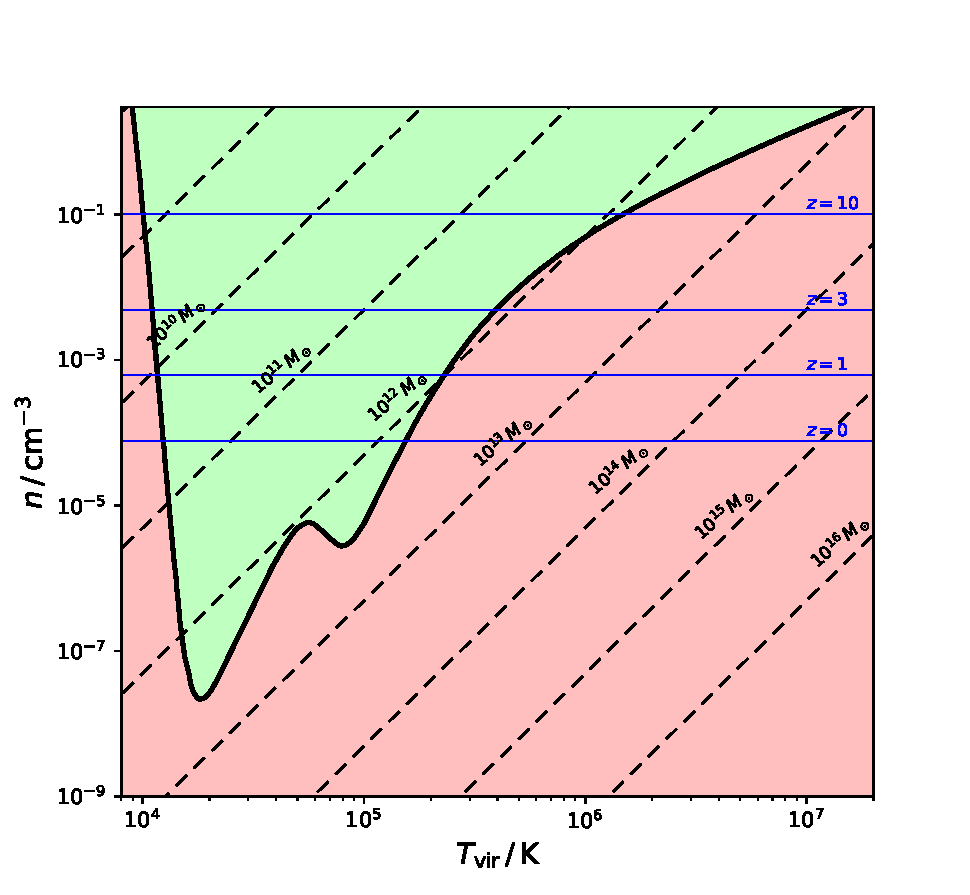
\includegraphics [width=0.48\textwidth] {cooling.pdf}
    \caption{Particle density $n$ as a function of virial temperature $T_\mathrm{vir}$. The black locus marks the values where the cooling timescale $t_\mathrm{cool}$ equals the dynamical timescale $t_\mathrm{ff}$. Above this curve, in the green region, clouds are able to cool sufficiently to spark star formation. Slanted, dashed lines show the $n\text{-}T_\mathrm{vir}$ values of halos with the indicated masses. Horisontal blue lines mark typical densities of virialized halos at the indicated redshifts.}
    \label{fig:cooling}
\end{figure}
The plot is divided into two regions showing where the cooling timescale is \emph{less than} (green) and \emph{greater than} (red) the free-fall timescale.
In the green domain, the gas collapses more or less freely with negligible thermal pressure while in the red domain, the cloud is pressure-supported in a quasi-static state where cooling can take longer than the Hubble time.

The shape of the $t_\mathrm{ff} = t_\mathrm{cool}$ locus (black) resembles the cooling function, with $n\propto (T/\Lambda)^{1/2}$, and is calculated assuming a metal-free gas. For a Solar metallicity cloud (i.e.~characterestic of the present-day Universe), cooling is more efficient by more than an order of magnitude in the $T \sim 10^{4.5\text{--}6.5}\,\mathrm{K}$ regime, but the low-density trough of the locus still lies at $M\sim10^{12}\,M_\odot$.
The slanted lines show densities and temperatures of halos of constant mass. We see that clouds of $M\sim10^{12}\,M_\odot$ can cool even at low densities while at higher and lower masses, cooling is less efficient.
In other words, the distribution of the galaxies' stellar masses --- the stellar mass function (SMF) --- should be suppressed on either side of $M\sim10^{12}\,M_\odot$; the mass of the Milky Way halo.
%At lower (higher) masses, the slope is shallower (steeper), resulting in a knee in the mass function where galaxies are most efficient at forming 

Converting from an observed LF to an inferred SMF is not straightforward, because the amount of light detected from a given amount of stars depends on many factors such the age of the stellar population, the metallicity, and interstellar dust.
In particular the short wavelengths are susceptible to dust, but also to age because the most massive and blue stars die out fast.
Therefore SMFs in infrared wavelengths are typically more robust than in the UV.
A discussion of the conversion from LFs to SMFs is beyond the scope of the current text, but can be found e.g.~in \citet{Song2016}.

The differential cooling explains why we should not expect the stellar mass function to simply mirror the HMF, shifted by the baryon fraction $f_\mathrm{b}$.
In the calculations of the region of efficient cooling in Fig.~\ref{fig:cooling} we assumed a halo overdensity of $\Delta=180$.
But this is the average overdensity inside the virial radius;
in reality the halo will have a decreasing density profile with much higher densities in the center, so at least some of the gas should be able to cool.

Taking into account the fact that gas accumulates and condensates in the bottom of the potential well created by the halo, \citet{White1978} calculated a LF.
The result was still that the typical galaxy is hosted by a $M_\mathrm{vir}\sim10^{12}\,M_\odot$ halo.
But now astronomers faced another nuisance:
The high density allowed galaxies to cool \emph{too} efficiently, vastly overpredicting the number density of especially small galaxies.

The rescue for this ``overcooling'' problem is believed be, mainly, three physical processes known as \emph{photoionization}, \emph{merging}, and \emph{feedback}.

\subsection{Photoionization}
\label{sec:reionization}

In the ``dark ages'', before the advent of the first luminous sources, the Universe was filled with neutral gas which absorbed all light blueward of the ionization threshold at $\lambda = 912\,{\AA}$ \citep{Gnedin2000,Barkana2001}.
Strong UV radiation created ionized bubbles around the first galaxies which percolated the Universe and eventually overlapped.
The resulting meta-galactic UV background permeates and heats the intergalactic medium (IGM) and increases its pressure, preventing accretion of gas onto halos, as well as reduced the rate of radiative cooling within the halos \citep{Benson2002}, inhibiting star formation.
Small halos are particular vulnerable to this effect, resulting in a shallower slope in the LF.
The UV background increased with time to a maximum and then decreased, with a characteristic value of $\Gamma\sim10^{-12}\,\mathrm{photons}\,\mathrm{s}^{-1}$, leading to a characteristic timescale for photoionization of $t_\mathrm{ph} \sim 1/\Gamma \sim 3\times10^4\,\mathrm{yr}$; much shorter than the typical dynamical timescales involved.

The exact timescales involved in this so-called ``epoch of reionization'' (EoR) are still not entirely clear:
What was its duration (when did it start and end; was it short and intense or more prolonged?), which sources contributed more (small galaxies, massive galaxies, or even quasars?),
and what was its topology (small and fizzly vs. large bubbles)?
%A major problem in calculating theoretically the course of the EoR is that it is highly non-linear and involves a huge dynamic range of spatial scales.

Analytical solutions exist for calculating the propagation of an ionized bubble around a source in a homogeneous gas, relating the output rate of ionizing photons to the timescale of recombination \citep{Stromgren1939,Dopita2003}.
Comparing these timescales, however, only puts weak constraints on the EoR; the largest advances in this field have been made through numerical simulations which can capture the highly non-linear nature of the involved densities, temperatures, velocities, etc.~\citep[see e.g.][for recent advances regarding the topology of reionization]{Hutter2020,Perez2022}.
A paramount problem in such calculations is the enormous range in spatial scales involved (see info box):
Typical bubbles have sizes of the order of ten(s of) Mpc \citep{Wyithe2004,Giri2018}, but photons begin ionizing gas already on sub-parsec scales, in the molecular clouds enshrouding the stars.
Most simulations have therefore had to focus either on the escape of ionizing radiation through the interstellar medium (ISM) of individual galaxies \citep[e.g.][]{Haid2019}, or on the ionization of the large scales of the intergalactic medium (IGM), regarding individual galaxies simply as (unresolved) photon sources \citep[e.g.][]{Jensen2013,Jensen2014}, although intermediate-scale simulations also do exist \citep[e.g.][]{Rosdahl2022}.

% \noindent\fcolorbox{darkgray}{lightgray}{%
\begin{figure}[!t]
\minipage[t!]{\dimexpr0.98\linewidth-2\fboxsep-2\fboxrule\relax}
\begin{bclogo}[
    couleur=gray!20,
    epBord=1,
    arrondi=0.1,
    logo=\bcinfo,
    marge=8,
    ombre=false, %true,blur,
    couleurBord=gray!60,
    barre=line]
    { \ \textsf{Dealing numerically with a multiplicity of timescales}}
    \small{\textsf{A fundamental challenge in numerical simulations --- not only in astrophysics --- is the vast dynamic range in both space and time.
    Computers are limited by both memory and processing power, and trade-offs must necessarily be made between simulating sufficiently large spatial and temporal scales, and resolving these scales sufficiently to capture the small-scale physics.
    Various approaches exist to alleviating these limitations; cosmological simulations, modeling a more or less representative chunk of the Universe, usually imploy an adaptive resolution.\vspace{1mm}\\
    Structures can be simulated using \emph{particles} that each represent a given amount of mass (gas, dark matter, and/or stars).
    This is analogous to simple $N$-body codes, but particles are ``smoothed'' in space \citep{Gingold1977,Lucy1977}.
    The particles follow trajectories dictated by forces (gravitational, hydrodynamical, magnetic, etc.), and resolution thus increases automatically in high-density regions.
    Alternatively, structure can be simulated on a fixed grid of cells, analogous to pixels in a picture but in 3D.
    Adaptive resolution can then be achieved by refining cells according to a pre-defined criterion (usually a density threshold), recursively splitting cells up in 8 cells \citep{Berger1984,Berger1989}.
    The two schemes both have their pros and cons.
    Additionally, a relatively new technique is a ``moving mesh'' that incorporates the best of two worlds; here space is split up into cells, but the cells have arbitrary (polyhedral) shapes, and they are not fixed in space but move around \citep{Springel2010}.\vspace{1mm}\\
    Not only space, but also time may be refined.
    In dense regions where matter undegoes large accelerations, numerical errors will be introduced if the time step is too big.
    In order to avoid wasting time \emph{when} matter is not dense, time steps may adapt to the density.
    Likewise, to avoid wasting time \emph{where} matter is not dense, different spatial domains may use different time steps such that the equations of motion are advanced first on the smallest time steps, and then on successively larger scales until the largest time step ``catches up'' with the smaller.
    }}
\label{info:adaptive}
\end{bclogo}
     \endminipage
     %}\hfill
\end{figure}

\subsection{Galaxy merging}
\label{sec:merging}

Even today, the separation between galaxies is not vastly larger than their cross section, and at $z\sim10$, where number densities were $10^3$ times larger, encounters between galaxies were frequent. Galaxies therefore interact gravitationally and occasionally merge with other galaxies. Minor mergers, where a galaxy of mass $M_1$ accretes a smaller galaxy of mass $M_2 \lesssim M_1/10$ are frequent at all times, but even major mergers events, with $M_1\sim M_2$, happen on average once per Hubble time \citep{Lacey1993}.
The effect of this process is to increase the number of large galaxies, at the expense of small galaxies \citep[e.g.][]{Cole1991,Kauffmann1993}.

To first order, the relevant timescale for accretion of satellite galaxies is set by a physical process known as \emph{dynamical friction}, described first by \citet{Chandrasekhar1943}, where the gravity of a large body moving through an ``atmosphere of collisionless gas'' (in this case the DM halo) creates a ``wake'' of increased mass, exterting a drag on the body.
%Merging takes place on the ``dynamical'' timescale $t_\mathrm{dyn}$, the relevant timescale for dynamical processes which is essentially the free-fall timescale to within factors of order unity.
For minor mergers, the timescale with which the orbit of a satellite decays decreases with increasing mass; \citet{Cole1994} found that a simple model with
\begin{equation}
    \label{eq:tmerge}
    t_\mathrm{merge} \sim t_\mathrm{dyn} \left( \frac{M_1}{M_2} \right)^{0.25},
\end{equation}
where the dynamical timescale $t_\mathrm{dyn}$ is essentially equal to the free-fall timescale, follows the trend of numerically simulated mergers.
For sufficiently large ratios between $M_1$ and $M_2$ (in this case if $M_2/M_1\gtrsim16$), the merging timescale exceeds the Hubble time, consistent with the fact that massive galaxies still have satellites today.
More sophisticated models \citep[e.g][]{Boylan-Kolchin2008}
%using the more appropriate dynamical timescale, which is essentially the free-fall timescale to within factors of order unity,
yield similar conclusions.

\subsection{Feedback}
\label{sec:feedback}

Even with the physical mechanisms described above, galaxy formation models struggled to match observed LFs, apparently producing too many stars.
This annoyance entailed the need for \emph{feedback} processes which could regulate star formation.
Early models \citep[e.g.][]{White1991,Somerville1999,Efstathiou2000} employed only supernova feedback which inject both thermal energy and momentum into the ISM. 
The efficacy of this process can be understood from a simple timescale perspective:
Star formation in galaxies occurs basically on the dynamical timescale which is of the order 100 Myr. In contrast, supernovae result from the explosions of the most massive stars which has life times of $\lesssim 10$ Myr.

Supernova feedback not only reheats the cold gas but may also expel it altogether in galactic ``winds'', and is thus very efficient at inhibiting star formation. The effect is particular pronounced in low-mass galaxies which have a shallower gravitational potential, allowing gas to escape more easily \citep{Dekel1986,Kauffmann1993,Natarajan1999}.
In fact, it turned out to be a bit too efficient, because the expelled gas then becomes available for accretion onto more massive halos (galaxy groups and clusters) where at late times it cools and forms galaxies much more massive than observed \citep{Benson2003}.

Various mechanisms were proposed to solve this problem of too many massive galaxies.
Arguably the most promising mechanism to prevent too many massive galaxies is feedback from active galactic nuclei --- that is, gas accreting onto supermassive black holes in the center of galaxies, radiating excess energy away at extreme energies.
This effect has been successful at matching LFs at low and high redshifts \citep[e.g.][]{Croton2006,Bower2006,Somerville2008,Mccarthy2011}.

\subsection{From halo mass to stellar mass}
\label{sec:hmf2smf}

The physical processes described in Secs.~\ref{sec:LF}--\ref{sec:feedback} are shown in Fig.~\ref{fig:hmf2smf}.
The blue line shows the HMF at $z=0.1$ (``almost today'').
It is a \citet{Sheth2002} HMF with a $z$-dependent correction factor which brings the analytical prediction very close to results from a large-scale, $\sim8$ billion particle, cosmological simulation \citep{Klypin2011};
its functional form is described in \citet{Laursen2019}.
Multiplying the mass by the cosmic baryon fraction $f_\mathrm{b}$ shifts the HMF to the left, shown by the black arrow.
If galaxies at all masses were able to cool and convert all their gas to stars, observed SMFs would look like the magenta line.
Reality is quite different: Observed SMFs at $z\sim0.1$ at the low-mass end \citep{Wright2017} and the high-mass end \citep{Bernardi2013} are shown with olive green and steel blue points, respectively.

The physical mechanisms thought to be responsible for this drastic suppression are indicated by the green and orange arrows.
The observations are compared to four different models that include these mechanisms: 
The brown lines show two semi-analytical models, GALFORM (\citealt{Gonzalez-perez2014}, but taken from \citealt{Somerville2015a}) and SAGE \citep{Croton2016}, while the cyan lines show results from numerical, hydrodynamical simulations, Illustris \citep{Vogelsberger2014} and EAGLE \citep{Schaye2015}.
While they are not perfect fits, all models are seen to capture rather well the shape of the SMFs.

The preceding discussion has illucidated how simple timescale arguments may both be helpful and provide insight into complex physical problems, but also have short-comings. In the final section, we will have a look at a contemporary problem in the context of galaxies where we are currently witnessing an apparent problem with the timescales of structure formation.

\begin{figure}[!t]
    \centering
    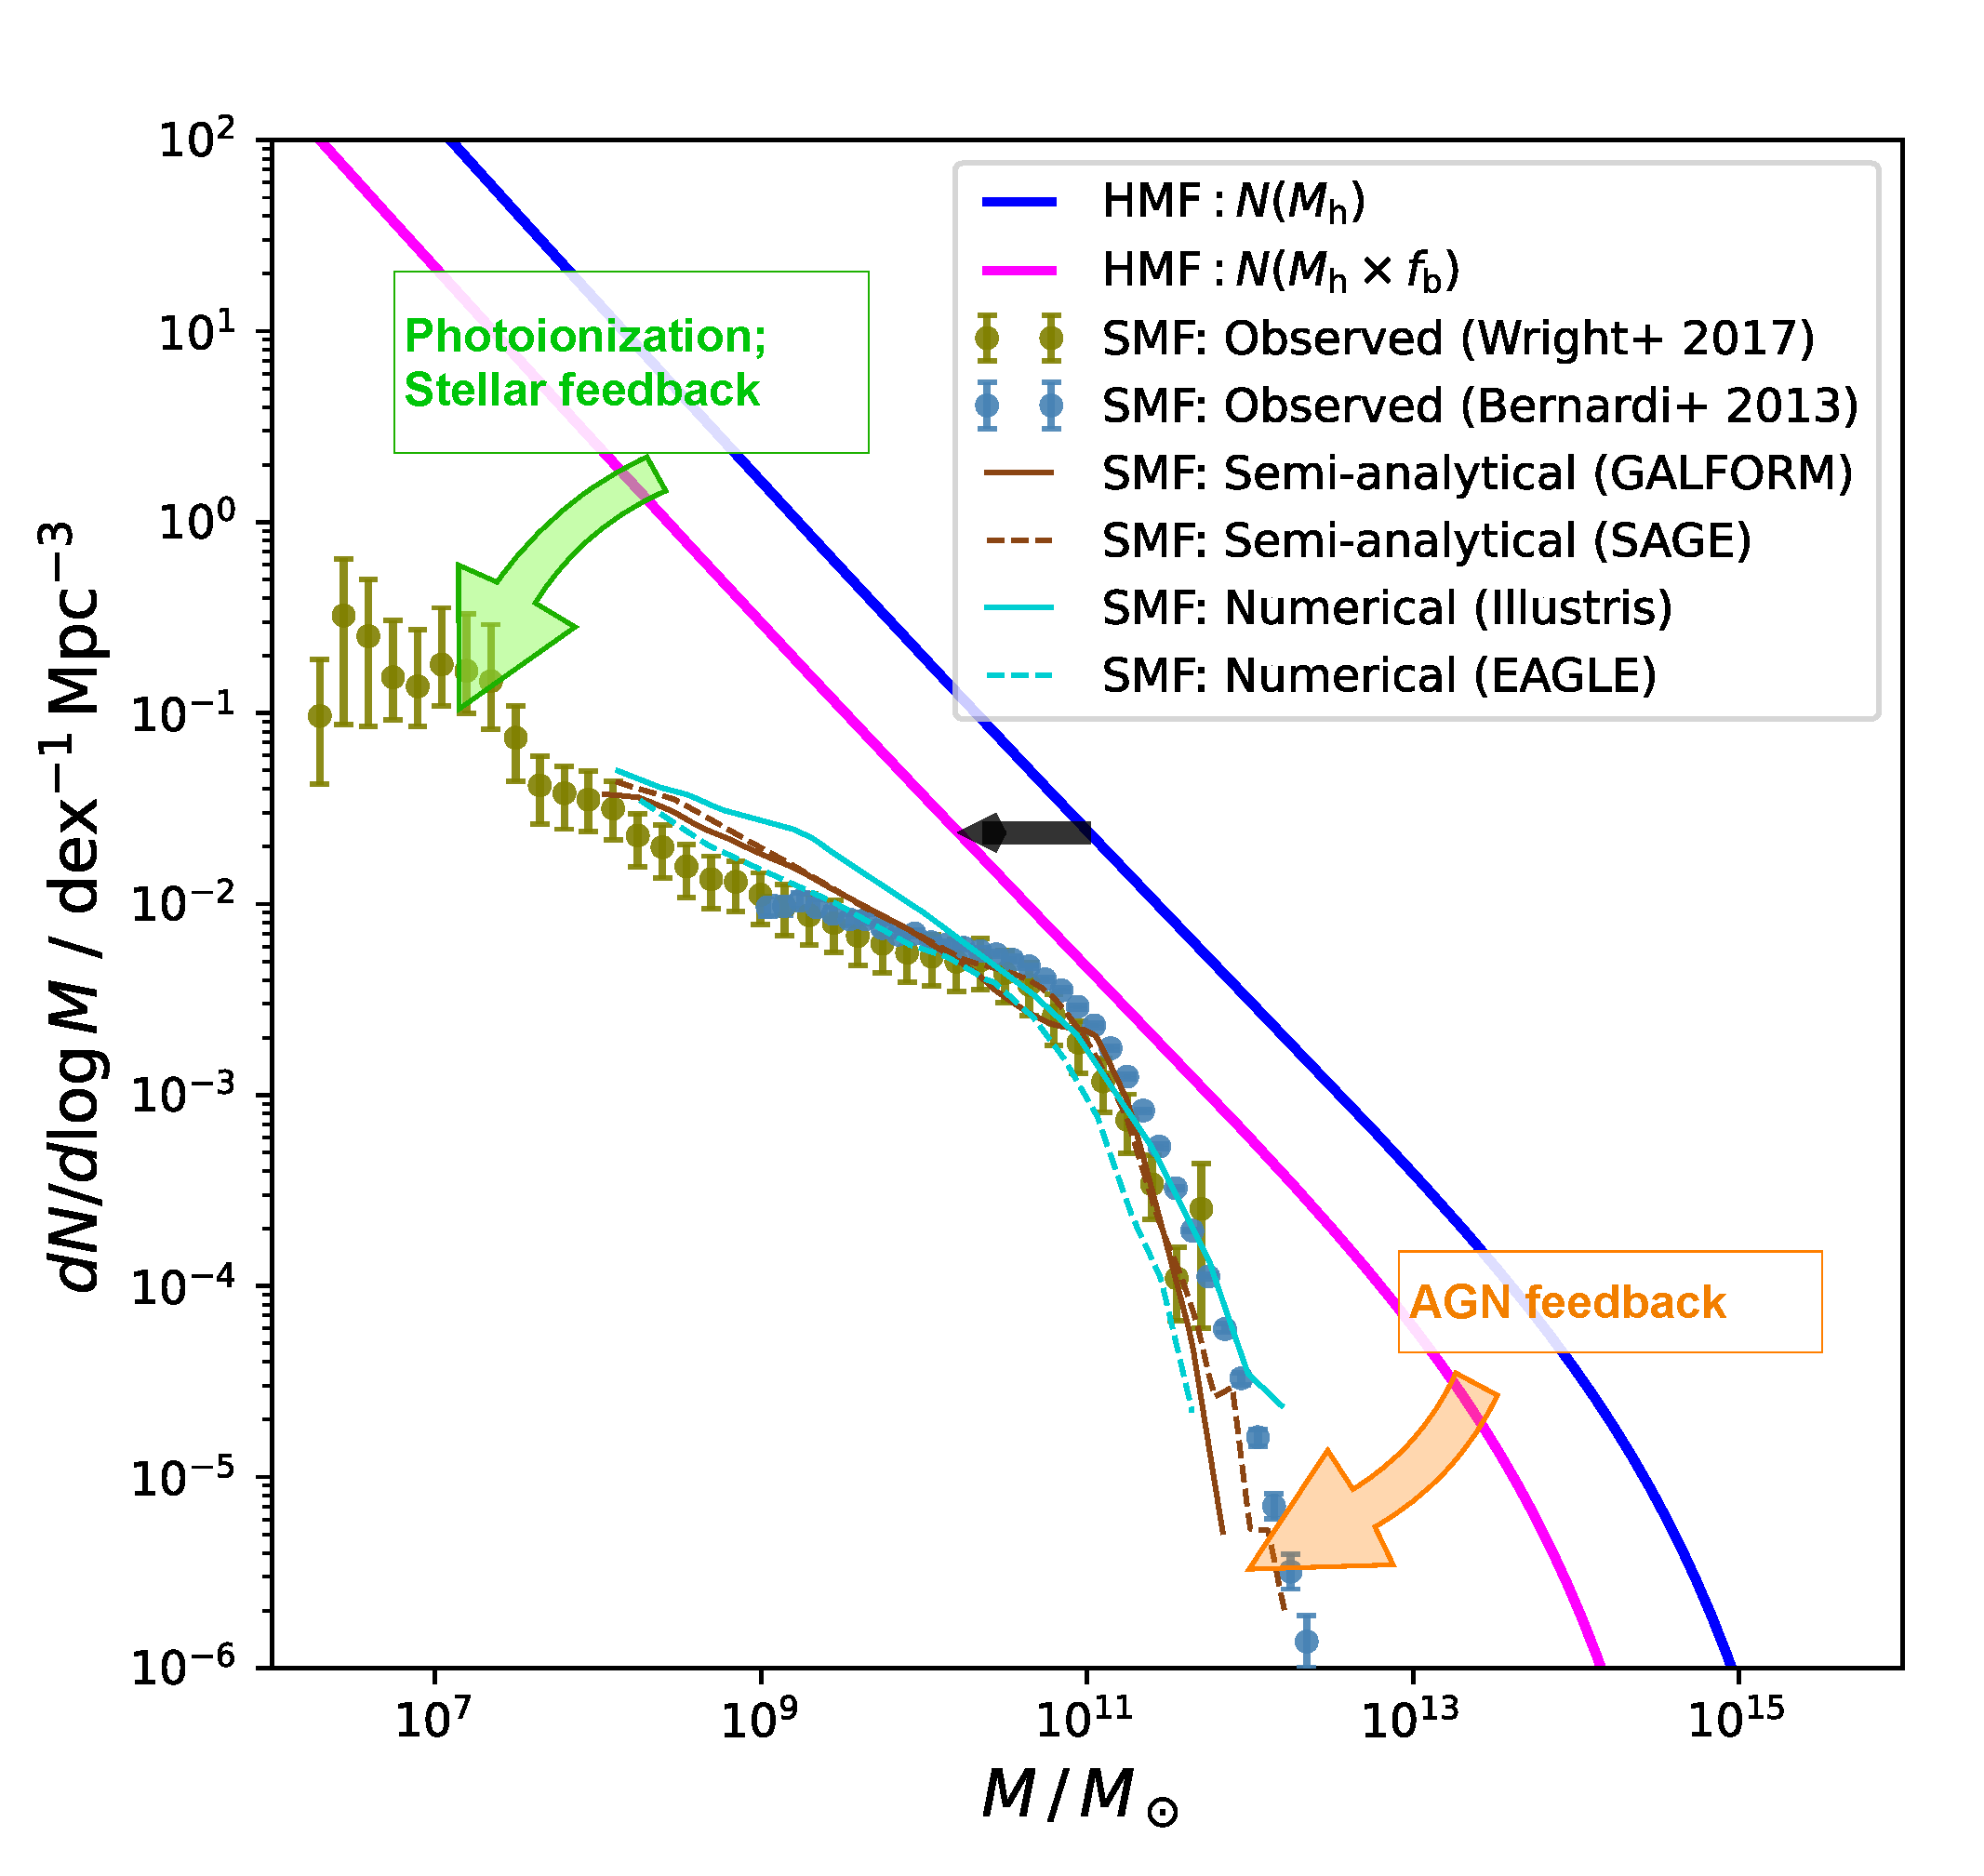
\includegraphics [width=0.48\textwidth] {hmf2smf-annotated.pdf}
    \caption{Number density of halo masses and stellar masses as a function of mass.
    Theoretical predictions from a HMF are shown in blue and magenta for total halo masses and corresponding baryon masses, respectively.
    Observed stellar mass functions at the low-mass end (olive) and high-mass end (steel-blue).
    Photoionization and stellar feedback is believed to suppress the mass function at the low-mass end (green arrow), while AGN activity suppresses the high-mass end (orange arrow).
    These mechanisms are incorporated in semi-analytical (brown) and numerical (cyan) models, which are seen to provide a reasonable match to the observations.}
    \label{fig:hmf2smf}
\end{figure}

\section{The first galaxies}
\label{sec:jwst}

On Christmas day 2021, we finally saw the successful launch of the long awaited James Webb Space Telescope (JWST).
Half a year later, after a month-long journey to its ``destination'' Lagrange point 2 (L2) 1.5 million kilometers from Earth, cooling to 6--40 K, adjusting its 18 mirror segments, as well as commissioning and calibrating of its four instruments, the astronomy community finally saw its science data in July 2022.
A proclaimed goal of JWST is to look for some of the very first galaxies, and it is therefore expected that we will eventually find galaxies with redshifts higher than the current ``record-holder'', GN-z11, which has a redshift of 11.09 \citep{Oesch2016} and is hence seen some 400 Myr after the Big Bang.

Finding the highest-redshift galaxy is not just a matter of breaking a record. The first luminous sources are thought to appear at a redshift of $z\simeq20\text{--}30$, when the Universe was 100--200 Myr old.
Although 100 Myr is not much, cosmologically speaking, finding a galaxy 300 Myr after the Big Bang is significantly closer to the epoch of first galaxies.
Figure~\ref{fig:zrecord} shows how our ``explored'' Universe has expanded, in terms of the most distant source detected.
\begin{figure}[!t]
    \centering
    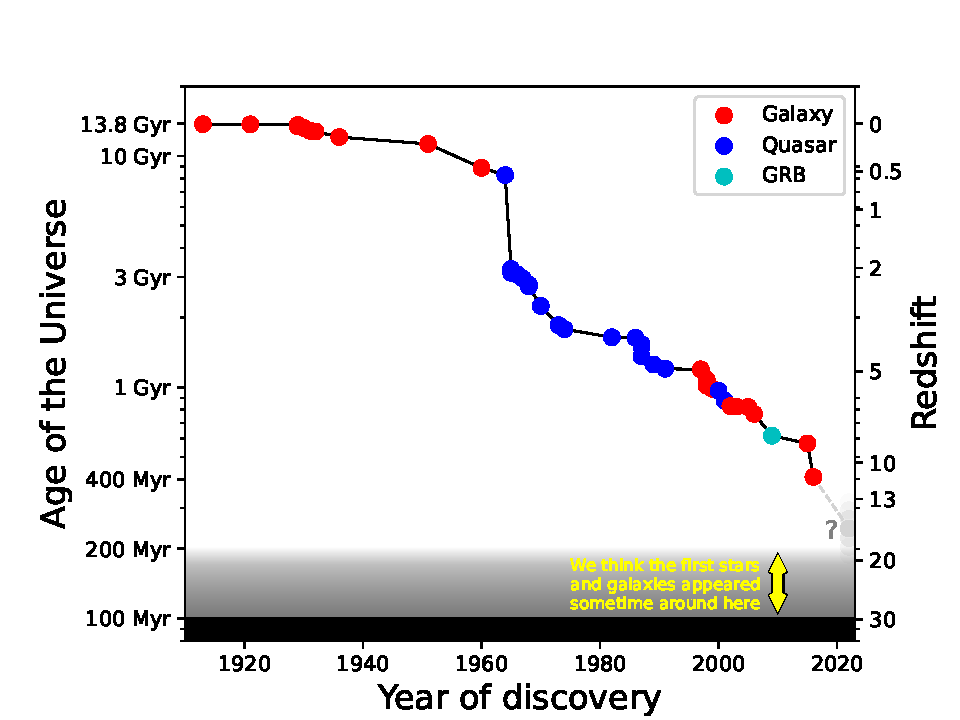
\includegraphics [width=0.48\textwidth] {zrecord.pdf}
    \caption{Earliest epoch at which an object in known (and the redshift of these objects on the right $y$ axis) vs.~the year of discovery.
    Most objects are galaxies (red), but from the mid-1960s to the mid-1990s, quasars (blue) were more easily found. The cyan point indicates the gamma-ray burst GRB 090423 \citep{Tanvir2009}.
    The still tentative $z=13.3$ galaxy HD1 \citep{Harikane2022a} has not been included, so the current record is set by GN-z11 at $z=11.09$.
    The gray extension indicates that this record is currently being challenged by reports of galaxies at $z=13\text{--}20$, approaching closely the epoch of advent of the very first luminous sources at $z\lesssim20$.}
    \label{fig:zrecord}
\end{figure}
The first galaxy to have its redshift measured (not counting the blueshifted Andromeda) was the Sombrero galaxy in 1913 with $z=0.004$ \citep{Slipher1915,Hoyt1980}. Progress was rather slow until the mid-1960s when it was realized that the bright point sources, first discovered as radio sources, were in fact extremely distant quasars \citep{Schmidt1964,Schmidt1965}
Because the timescales for building up the supermassive black holes needed for a quasar to form is at least a few $10^8$ years, these object become increasingly rare as we go to higher redshifts, and above $z\sim6$ astronomers had to wait for new techniques to discover high-redshift galaxies.
Rescue came with the so-called dropout technique \citep{Steidel1996} which since the mid-1990s has resulted in a steadily increasing highest redshift.

No more than five days after science data started flowing from JWST, the first reports of a redshift record-breaking galaxy came, when \citet{Naidu2022a} announced, on the preprint server arXiv, the discovery of two galaxies with apparent redshifts of $z\simeq11$ and $z\simeq13$, dubbed GLASS-z11 and GLASS-z13, respectively.
Simultanteously\footnote{In fact uploaded to arXiv a mere 2:02 minutes after the Naidu paper.} with this, \citet{Castellano2022} reported a sample of galaxies with redshifts up to $z\simeq15$.
In the days to follow, more astounding discoveries came, with galaxies at
$z\sim17$ \citep{Donnan2022,Harikane2022}, and even
$z\sim20$ \citep{Yan2022}.
Could this really be some of the very first galaxies, consisting of stars made of pristine gas?

What is even more remarkable is that the galaxies seemingly are exceptionally massive; indeed the inferred stellar masses are much higher than expected to be physically possible from our understanding of hierarchical clustering and galaxy assembly.
The $z\simeq17$ galaxy, CEERS-1749, has a stellar mass of almost $10^{10}\,M_\odot$, a tenth of the Milky Way.

Figure~\ref{fig:jwst} shows the four galaxies mentioned above --- GN-z11, GLASS-z11, GLASS-z13, and CEERS-1749 --- in a stellar mass vs.~age of the Universe plot. The blue line shows the maximum expected mass of a galaxy at a given time in the volume surveyed, if 1) we allow galaxies at that time to be 100\% efficient at converting gas to stars (which is a factor of at least 10 more efficient than in the more nearby Universe), and 2) we assume that the standard model of the structure and evolution of the Universe, the so-called $\Lambda$CDM model, is correct.
Above this line, in the red domain, galaxies are unlikely to have been able to build up so much mass, while in the green domain we should not be too surprised to find galaxies.
\begin{figure}[!t]
    \centering
    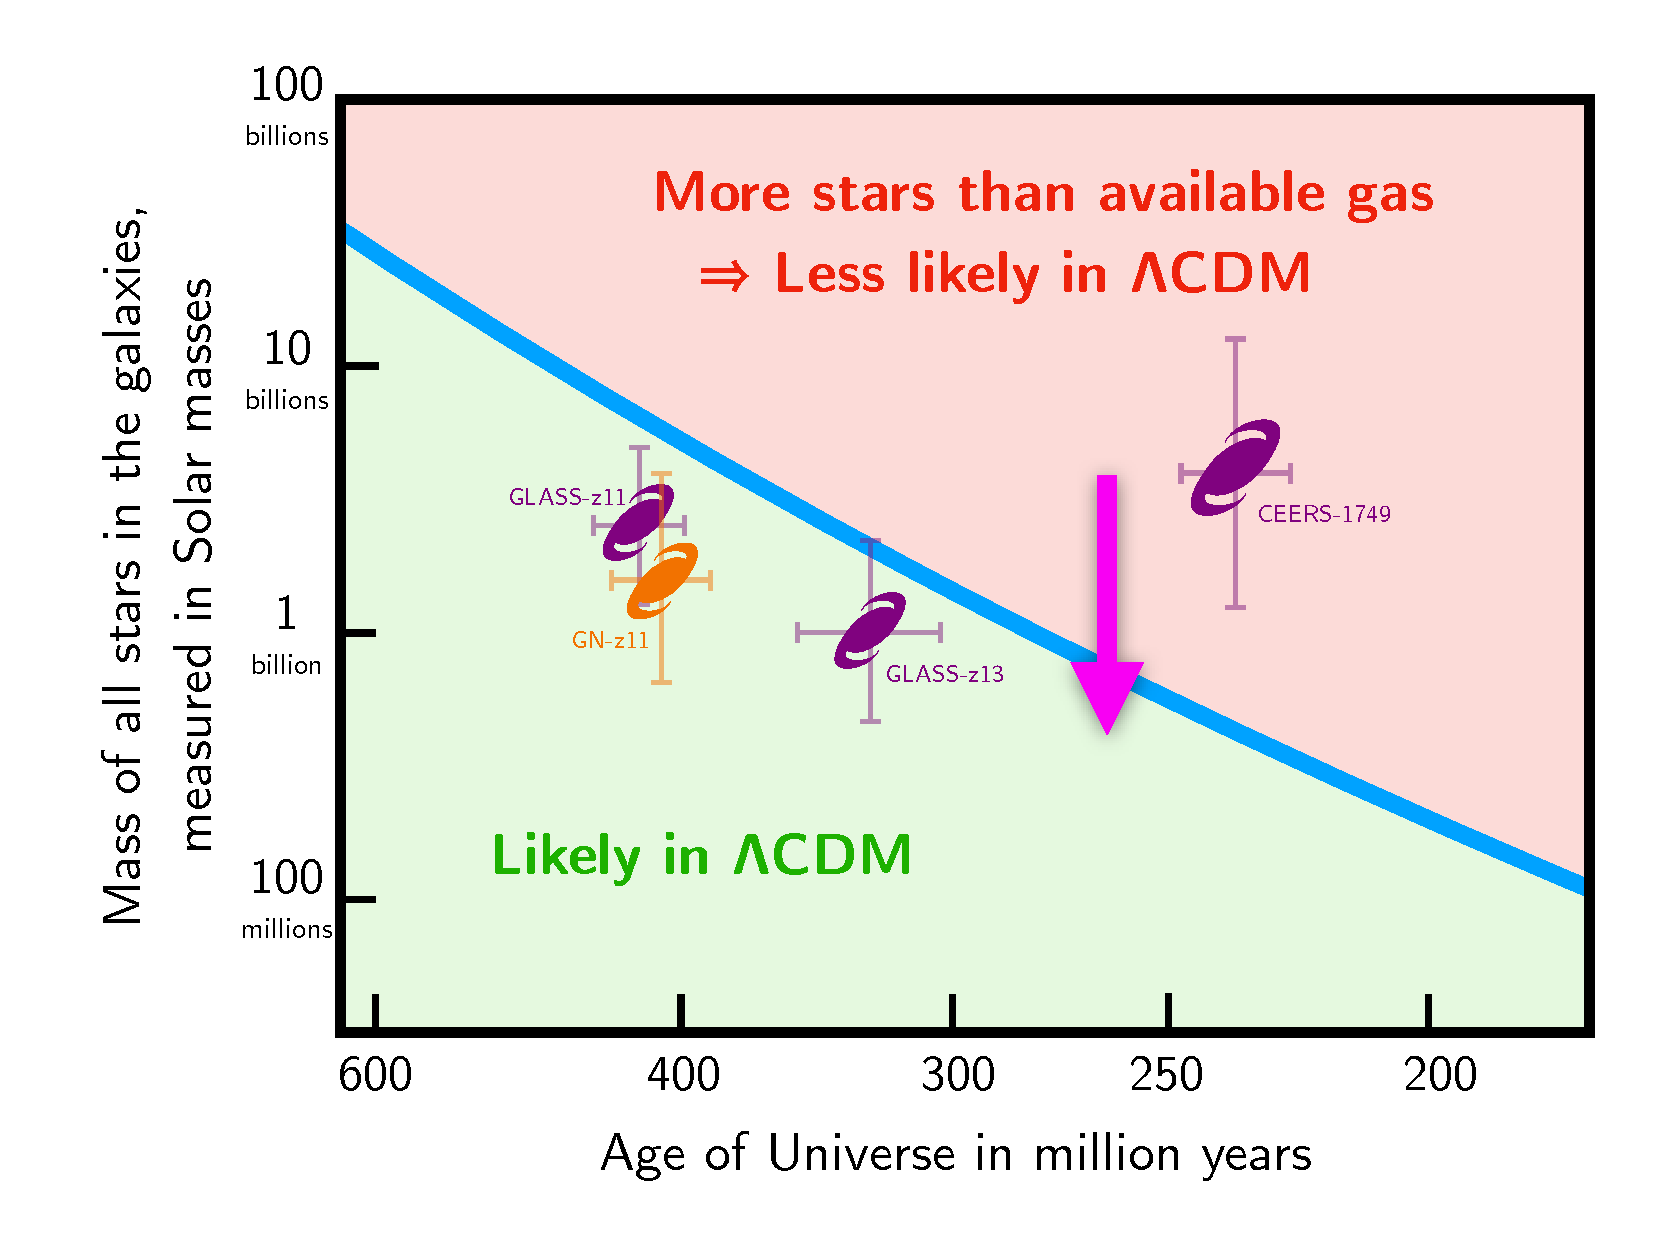
\includegraphics [width=0.48\textwidth] {jwst.pdf}
    \caption{Stellar masses of some galaxies recently observed with JWST, vs.~the age of the Universe at the time we see them.
    The blue line divides the ``likely'' region from the ``unlikely'' under the current $\Lambda$CDM paradigm, assuming a 100\% star formation efficiency, i.e.~ with $M_*/M_\mathrm{halo} = f_\mathrm{b}$.
    The magenta arrow show how far down all galaxies would move assuming a temperature-dependent initial mass function of newborn stars, which produces brighter stars on average, and hence leads to a smaller inferred stellar mass for a given luminosity.
    The figure is based on Fig.~5 from \citet{Naidu2022b}.}
    \label{fig:jwst}
\end{figure}
Three of the galaxies are on the verge of being probable (if we assumed a star formation efficiency similar to lower redshifts) while CEERS-1749 seemingly defies the timescales of $\Lambda$CDM.
Had we instead assumed a star formation efficiency similar to the more nearby Universe, the blue line would fall below all four galaxies.

Before claiming that not the the redshift record, but also $\Lambda$CDM has been broken, there are however a number of caveats that must be considered.
First of all, at the time of writing this text, the papers have not yet been peer-reviewed.
More importantly, the method by which the redshifts have been measured is a somewhat unreliable way. None of them have spectra, which would be needed to measure exact redshifts. Instead the redshifts are estimated through the ``drop-out technique'': At these high redshifts, the Universe is predominantly neutral (we are deep in the epoch of reionization), so all light blueward of the Lyman break at $912\,{\AA}$ is absorbed, and galaxies will appear black in --- or \emph{drop out} of --- images taken with filters blueward of this break.
The higher the redshift a galaxy has, the redder the filter it will drop out of, so imaging a field with multiple filters gives a crude estimate for the redshift.

Not only is the redshift imprecise; without a spectroscopical redshift to confirm spectral features, we cannot be certain that the galaxy is not red for some other reason than redshift. Dusty galaxies also appear red, because dust absorbs more easily shorter wavelengths. Galaxies with old stellar populations, where the massive blue stars have died, similar appear red. Even brown dwarfs in the Milky Way may sometimes allude the observer.
For this reason the galaxies must be followed up spectroscopically (an indeed will be soon).

Many other explanations have also been proposed for the too-bright galaxies.
\citet{Mason2022} showed that stochastic star formation, where stars sometimes form slowly and other times fast, as well as more dust-free environments, could make a fraction of the galaxies appear much brighter than average, and that we are seeing ``the tip of the iceberg''.
There is also the possibility that we have simply been lucky and pointed the telescope in a fortunate direction with galactic overdensities.
\citet{Steinhardt2022} point out that the templates that are used to calculate redshifts from the series of images through different filters are based on physics known from the local Universe. But there are several reasons to believe that this is not appropriate at very high redshifts. For instance they argue that, because the Universe was hotter in the past, the mass distribution of stellar populations was significantly different from today.
As demonstrated by \citet{Sneppen2022}, accounting for the different gas temperature in the early Universe, the calculated masses of the galaxies seems to be significantly smaller, probably at least ten times.
In other words, the galaxies in Fig.~\ref{fig:jwst} would move down at least by an amount indicated by the magenta arrow, placing them in the more likely (green) domain.
More possible explanations are discussed in recent papers such as \citet{Kannan2022}.

Even prior to JWST, some of the highest-redshift galaxies were in tension with the current paradigm, described by \citet{Steinhardt2016} as the ``impossible early galaxy problem''.
But although at first glance the observations from JWST seem difficult to reconcile with the timescales of structure formation, there are still many things to consider before claiming the downfall of $\Lambda$CDM.

\section{Conclusion}
\label{sec:conclusion}

Modeling the multiplicity of timescales in astrophysical systems is challenged by the immense span; from sub-second processes to gigayears.
Nevertheless, this span can in some cases be an advantage in that one may simply compare characteristic timescales involved in the processes to predict their outcome.
In this chapter, we have reviewed the physics of galaxy formation and seen how timescales regulate which dark matter halos are able to form galaxies, and how efficient they are at forming stars.

As a more contemporary topic, we have discussed the recent reports of ``impossibly early galaxies'', and how they are in tension with the timescales of early structure formation.
The $\Lambda$CDM model has been extremely successful not only as an explanation of existing observations, but also in making predictions such as weak gravitational lensing \citep{Fischer2000}, CMB polarization \citep{Kovac2002}, and patterns in the large-scale structure of the matter distribution
%; the so-called \emph{baryonic acoustic oscillations}
\citep{Eisenstein2005}.
However, the model builds upon three somewhat unstable pillars, namely general relativity which despite its success on large scales is yet to be unified with quantum mechanics, and dark matter and dark energy, the nature of which is unknown and even questioned by a significant fraction of the scientific community.
While it is thus not at all unlikely that we will at some point have to face a cosmological paradigm shift, there are many reason to wait making too strong statements about $\Lambda$CDM; we will have to await more data, in particular spectroscopic data and more wide-field surveys.

\begin{center}
\pgfornament[width=.4\textwidth]{89}
\end{center}

\begin{acknowledgements}
    I am grateful for fruitful discussions with Charles L.~Steinhardt and Steen H.~Hansen.
    The Cosmic Dawn Center (DAWN) is funded by the Danish National Research Foundation under grant No. 140.
\end{acknowledgements}

\bibliographystyle{aa}
\bibliography{timescales}
\end{document}
